\capitolo{Controllo del Moto in presenza di Gioco}
Il gioco è caratterizzato da una variazione dell'inerzia equivalente legata a cambio di segno di \(T_2\) (questo non si verifica in ogni situazione, vedi {\color{red} Riferimento quando nelle viti a ricircolo si parlò di gioco}). 
Motore e carico possono essere accoppiati per fianco destro o sinistro perciò \(J_{eq} = J_m + \tau^2 J_c\); motore e carico possono essere disaccoppiati \(J_{eq} = J_m\).

\sezione{Problema del gioco}
Il problema legato alla variazione di inerzia è il seguente:
\[
\begin{cases}
    \text{Accoppiati: } J_{eq} = J_m (1+\rho) \ \rightarrow \ \omega_{bv}^{min} \simeq \frac{K_{pv}K_T}{J_m(1+\rho)} \\
    \text{Disaccoppiati: } J_{eq} = J_m \ \rightarrow \ \omega_{bv}^{max} \simeq \frac{K_{pv} K_T}{J_m}
\end{cases}
\]
Ossia passando da carico e motore accoppiati a disaccoppiati, per \(K_{pv}\) costante, la banda passante varia di un fattore \(1+\rho\), l'aumento di banda passante è associato a avvicinamento a \(\omega_I,\omega_{tv}\), che potrebbe portare a calo di margine di fase, e instabilità.

Il gioco è caratterizzato da passaggio imprevedibile da motore carico accoppiati e disaccoppiati, e il cambio tende ad autoalimentarsi, si instaura un ciclo limite di oscillazione non armonica permanente.
Questo problema affligge controllo colocato e non colocato.

\sottosezione{Soluzioni}
Una possibile soluzione è \textbf{riduzione di rapporto di inerzia}, così facendo la differenza di inerzia tra c-m disaccoppiati/accoppiati è minore, le bande passanti e i margini di fase risultano simili.
Tuttavia la scelta di \(\rho\) non dovrebbe portare a utilizzo di riduttori con alto rapporto di trasmissione e gioco elevato.

\begin{figure}[h]
    \centering
    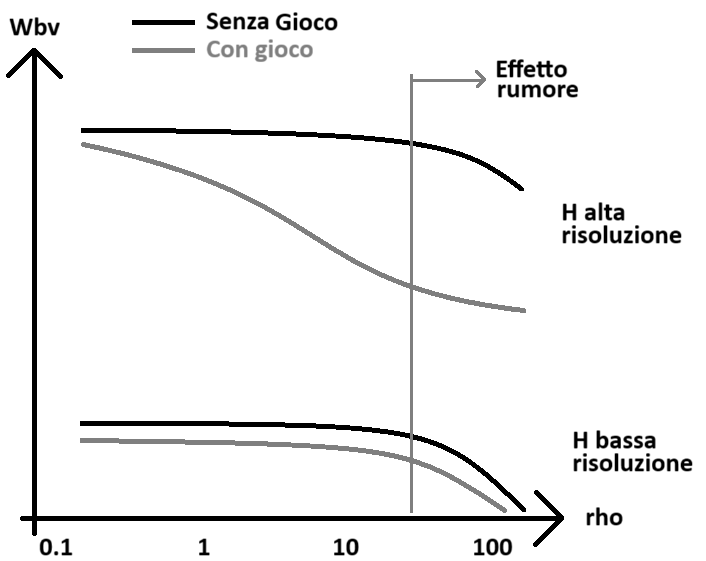
\includegraphics[width=0.45\textwidth]{Immagini/gioco_banda_passante_rho.png}
    \caption{Effetto del gioco: \(\omega_{bv}(\rho)\)}
\end{figure}

%% perchè la curva grigio scuso con H alta ha quella forma, ho scritto "legata al gioco per garantire omega_bv^max < limite", ma che significa?

In alternativa \textbf{riduzione} \(\mathbf{K_{pv}}\), dimensionata in modo da ottenere \(\omega_{bv}^{max} < \omega_{bv}^{lim}\) o comunque tale da garantire un certo margine di fase\footnote{La scelta del margine di fase non dovrebbe essere eccessivamente conservativa, \(m_\phi = 20^\circ\), serve per evitare l'autoalimentazione, dovrebbe servire un numero ridotto di volte per ciclo.} anche per c-m disaccoppiati.
